\documentclass[12pt]{article}

\usepackage[utf8]{inputenc}
\usepackage[T1]{fontenc}
\usepackage[margin=1in,top=1in,bottom=0.5in]{geometry}
\usepackage{newtxtext,newtxmath}
\usepackage{setspace}
\usepackage{graphicx}
\usepackage{subcaption}
\usepackage{booktabs}
\usepackage{longtable}
\usepackage{amsmath}
\usepackage{hyperref}
\usepackage{tikz}
\usetikzlibrary{arrows.meta,positioning}
\usepackage{microtype}
\usepackage{placeins}
\usepackage{fancyhdr}

\setstretch{1.15}
\setlength{\parindent}{0pt}
\setlength{\parskip}{\baselineskip}
\setlength{\emergencystretch}{2em}

\pagestyle{fancy}
\fancyhf{}
\fancyhead[R]{\thepage}
\renewcommand{\headrulewidth}{0pt}

\usepackage[
  backend=biber,
  style=numeric-comp,
  sorting=none,
  doi=true,
  url=true,
  maxnames=6,
  minnames=6
]{biblatex}
\renewcommand*{\mkbibbrackets}[1]{(#1)}
\addbibresource{references.bib}

\hypersetup{
  colorlinks=true,
  linkcolor=black,
  citecolor=black,
  urlcolor=blue
}

\newcommand{\PaperTitle}{Predicting MEN2-Associated Medullary Thyroid Carcinoma in RET Carriers: A Reproducible Machine Learning Pipeline}

\begin{document}

\begin{titlepage}
\centering
\vspace*{\fill}
{\Large\bfseries \PaperTitle\par}
\vspace{1.5cm}
{\large Harnoor Kaur$^{a}$, Arjun Vijay Prakash$^{a}$, Shashwat Mishra$^{a*}$\par}
\vspace{1.0cm}
$^{a}$ City Montessori School, Kanpur Road, Lucknow, Uttar Pradesh, India.\par
E-mail: \href{mailto:har.nooor16@gmail.com}{har.nooor16@gmail.com} (H. Kaur); \href{mailto:arjunv.prakash12345@gmail.com}{arjunv.prakash12345@gmail.com} (A. V. Prakash); \href{mailto:mishra.shashwat4002@gmail.com}{mishra.shashwat4002@gmail.com} (S. Mishra, corresponding author)\par
\vfill
\end{titlepage}

\setcounter{page}{1}

\section*{Abstract}
Multiple Endocrine Neoplasia syndrome type 2 (MEN2) is a rare hereditary endocrine cancer syndrome caused by germline mutations in the proto-oncogene REarranged during Transfection (RET). MEN2 is clinically associated with medullary thyroid carcinoma (MTC) and may also involve pheochromocytoma and primary hyperparathyroidism; biochemical evaluation often includes serum calcitonin and carcinoembryonic antigen (CEA), which are frequently elevated in MTC \cite{doi_10_1089_thy_2014_0335}.

A key barrier in resource-limited settings is access to confirmatory RET genetic testing, which can be cost-prohibitive for many families. We address this gap by developing a reproducible machine learning workflow for screening-oriented risk stratification using routinely reported clinical features and biomarkers. The prediction task is binary classification of MTC status (MTC vs.\ no MTC) in literature-derived MEN2/RET-carrier cohorts, intended to support prioritization and follow-up rather than replace genetic diagnosis.

Patient-level data were curated from published case reports and cohorts, yielding 152 confirmed RET carriers across 20 peer-reviewed studies spanning 24 RET variants and ATA risk levels 1--3. Key inputs include demographic and presentation variables, RET variant and risk level (when known), and biomarkers including calcitonin and CEA.

We implemented a pipeline that harmonizes heterogeneous sources, imputes missing CEA values using Multiple Imputation by Chained Equations with Predictive Mean Matching (MICE+PMM), engineers variant-aware interactions, benchmarks five model families (logistic regression, random forest, LightGBM, XGBoost, and linear SVM) under stratified validation with Synthetic Minority Over-sampling Technique (SMOTE) applied to training folds, and automatically quantifies uncertainty through bootstrap confidence intervals (1,000 iterations).

On the original paper-only cohort, logistic regression achieved 100\% recall (zero missed cancers) with 70.97\% accuracy. In the case-control setting (n = 1{,}069 total records), LightGBM achieved the highest accuracy (97.20\%) with 96.08\% recall. These results support MEN2 Predictor as a screening and risk-stratification aid to complement genetic testing and clinical guidelines, with prospective validation required prior to clinical deployment.

\section*{Keywords}
MEN2; RET; Medullary thyroid carcinoma; Calcitonin; Carcinoembryonic antigen; Rare disease; Machine learning; Screening; Risk stratification; Reproducibility

\clearpage

\section{Introduction}
Multiple Endocrine Neoplasia (MEN) syndromes are hereditary endocrine disorders classically categorized as MEN1, MEN2, and MEN4. MEN2 is caused by germline mutations in the proto-oncogene RET and is clinically subdivided into MEN2A, MEN2B, and Familial Medullary Thyroid Carcinoma (FMTC). The central clinical threat across MEN2 subtypes is medullary thyroid carcinoma (MTC), a potentially fatal malignancy arising from parafollicular C-cells. MEN2A commonly involves MTC and may also present with pheochromocytoma and primary hyperparathyroidism; MEN2B is associated with aggressive MTC and pheochromocytoma and may include non-endocrine manifestations; and FMTC is typically characterized by MTC with limited extra-thyroid features \cite{doi_10_1089_thy_2014_0335}.

\subsection{Problem and Proposed Solution}
Definitive diagnosis and cascade screening rely on genetic assays (e.g., Next Generation Sequencing or Sanger sequencing of RET exons), which can remain cost-prohibitive in resource-limited settings. In India, testing commonly ranges from approximately INR 19{,}000--20{,}000, limiting access for many families. This creates a practical gap between clinical suspicion and confirmatory genotyping, especially when biomarker monitoring (e.g., calcitonin and CEA) or imaging suggests elevated risk.

Our goal is to translate published clinical observations into an accessible, reproducible machine learning workflow that supports screening-oriented risk stratification. Rather than replacing genetic diagnosis, the intended use is to aid prioritization and follow-up by estimating the likelihood of MTC given available clinical presentation features and biomarkers, and to benchmark how augmentation strategies affect sensitivity in a safety-critical setting.

\subsection{Related Work}
Clinical decision-making for MEN2 is guided by genotype--phenotype correlations and evidence-based management recommendations, including biomarker-informed surveillance and intervention thresholds \cite{doi_10_1089_thy_2014_0335}. In contrast, machine learning for MEN2 is limited by the rarity of the condition and the lack of large, standardized datasets. Most published evidence consists of heterogeneous case reports and small cohorts, which are valuable for mechanistic insight but challenging for reproducible model training and evaluation.

\subsection{Challenges}
Rare-disease modeling introduces several challenges: small sample size, heterogeneous reporting across sources, incomplete biomarker measurements, and class imbalance between MTC and non-MTC cases. These issues can inflate apparent accuracy, destabilize sensitivity, and complicate fair model comparison. Additionally, synthetic augmentation can improve accuracy yet introduce clinically unacceptable recall volatility. MEN2 Predictor is designed to surface these trade-offs through a transparent pipeline with explicit evaluation on both the original paper-only cohort and an expanded case-control setting.

\section{Materials and Methods}

\subsection{Data Sources}
This study is a retrospective secondary analysis of published, de-identified, patient-level data extracted from twenty peer-reviewed studies \cite{doi_10_1210_jcemcr_luaf002,doi_10_3390_genes13050864,doi_10_1186_s12887_020_02224_4,doi_10_1016_j_ando_2015_10_007,doi_10_1007_s00595_013_0826_8,doi_10_1097_MS9_0000000000002923,doi_10_1155_2012_491054,doi_10_1155_2020_4147097,doi_10_3390_clinpract14060179,doi_10_1530_EDM_24_0009,doi_10_4103_ijc_IJC_639_19,doi_10_1210_jc_2015_2948,doi_10_12998_wjcc_v12_i15_2627,doi_10_1089_thy_2016_0374,doi_10_1530_eje_1_02216,doi_10_1210_jc_2017_02402,doi_10_18632_oncotarget_4992,doi_10_12659_AJCR_935207,doi_10_1210_clinem_dgac222}. The paper-only dataset contains 152 confirmed RET carriers across 24 variants with the binary target label MTC vs. no MTC.

\subsection{Policy and Ethics}
No new human participants were recruited and no animal experiments were conducted. The analysis uses only secondary data derived from published studies without additional identifiable patient information. Institutional review board approval was not required for analysis of published, de-identified secondary data.

\subsection{Statement of Informed Consent}
Informed consent was not obtained for this analysis because it did not involve direct interaction with participants; consent and ethics approvals (where applicable) were handled by the original studies.

\subsection{Feature Construction}
The pipeline constructs demographic, genetic, biomarker, and clinical features including age, sex, RET variant (one-hot encoded), ATA-aligned variant risk level, calcitonin and CEA measurements (with missingness indicators), thyroid ultrasound nodule features, family history of MTC, pheochromocytoma, and hyperparathyroidism.

\subsection{Biomarker Integration and Imputation}
CEA missingness is handled using multivariate imputation by chained equations with predictive mean matching \cite{doi_10_18637_jss_v045_i03}. The imputation model is informed by 34 observed paired calcitonin--CEA measurements across twelve cohorts (including a ctDNA cohort contributing 16 pairs). The observed calcitonin--CEA Pearson correlation is 0.2425 (n = 34), and the imputation strategy is applied after cohort assembly to preserve reproducibility.

\subsection{Datasets: Paper-Only and Expanded Case-Control}
Two datasets are evaluated:
(i) \textbf{Original (paper-only)}: the 152-carrier cohort.
(ii) \textbf{Case-control}: the original cohort augmented with variant-matched synthetic controls and trained with SMOTE class balancing applied only to the training split \cite{doi_10_1613_jair_953}. The case-control dataset comprises 1{,}069 total records.

\subsection{Models}
Five models are benchmarked: logistic regression, random forest, linear support vector machine (SVM), XGBoost \cite{doi_10_1145_2939672_2939785}, and LightGBM \cite{ke2017lightgbm}. Model training and evaluation follow a standardized pipeline implemented with scikit-learn \cite{pedregosa2011scikit}.
Logistic regression is used as the linear baseline model to estimate the probability of MTC from the engineered feature vector.

\subsection{Code Availability}
The pipeline, data artifacts, and figure-generation scripts are available in the GitHub repository: \url{https://github.com/arjuncodess/men2-predictor}.

\subsection{Training and Statistical Approach}
Each dataset is split using an 80/20 stratified train/test partition with fixed random seed (random\_state = 42). Hyperparameter tuning is performed via cross-validation on the training split, and SMOTE is applied only to the training data to mitigate leakage. Performance metrics include accuracy, precision, recall (sensitivity), F1-score, ROC-AUC, and average precision. Uncertainty quantification through 95\% bootstrap confidence intervals (1{,}000 iterations) is automatically performed for all models. Recall stability between original and expanded workflows is evaluated using permutation testing (10{,}000 shuffles); McNemar's test is not applicable because positive cases differ between the original and expanded test sets.

\section{Results and Discussion}

\subsection{Cohort Summary}
The paper-only cohort includes 152 RET carriers across 20 studies, with 72 MTC cases and 107 females / 45 males. Mean age is 35.44 years (median 34.0; range 1--90).

\begin{table}[ht]
\centering
\caption{Summary of the paper-only cohort (n = 152 RET carriers).}
\begin{tabular}{@{}ll@{}}
\toprule
Characteristic & Value \\
\midrule
Studies included & 20 \\
Total carriers & 152 \\
RET variants & 24 \\
MTC cases & 72 \\
Female / Male & 107 / 45 \\
Age (mean; median; range) & 35.44; 34.0; 1--90 \\
Observed calcitonin--CEA pairs & 34 (12 cohorts) \\
\bottomrule
\end{tabular}
\end{table}

\subsection{Screening-Safe Baseline on Paper-Only Data}
On the paper-only test split (31 patients), logistic regression achieves 100\% recall (sensitivity) with 70.97\% accuracy. In safety-critical screening, sensitivity is prioritized because each incremental loss in recall corresponds to a missed cancer case in the tested cohort.

\subsection{Effect of Synthetic Augmentation}
Synthetic expansion increases accuracy substantially for ensemble models, with LightGBM achieving 97.20\% accuracy and 96.08\% recall on the expanded test split (44 patients). Relative to the paper-only baseline, augmentation can reduce recall for some models; permutation testing did not detect statistically significant recall drops under the study's test-set structure.

\begin{table}[ht]
\centering
\caption{Test-set accuracy and recall (sensitivity) for original (paper-only) and expanded datasets.}
\begin{tabular}{@{}lcccc@{}}
\toprule
Model & Acc (Original) & Recall (Original) & Acc (Expanded) & Recall (Expanded) \\
\midrule
Logistic Regression & 0.7097 & 0.8667 & 0.7944 & 0.9804 \\
Random Forest & 0.8065 & 0.9333 & 0.9346 & 0.9608 \\
LightGBM & 0.8065 & 0.8667 & 0.9720 & 0.9608 \\
XGBoost & 0.7419 & 1.0000 & 0.8738 & 0.9804 \\
SVM (Linear) & 0.6452 & 1.0000 & 0.4626 & 0.9804 \\
\bottomrule
\end{tabular}
\end{table}

\subsection{Interpretability}
The pipeline computes SHAP attributions \cite{lundberg2017shap} for supported models and provides per-model feature-importance summaries. In the expanded LightGBM model, genotype and biomarker features jointly contribute to risk stratification, consistent with clinical expectations that risk depends on both variant class and biochemical phenotype.

\begin{figure}[ht]
\centering
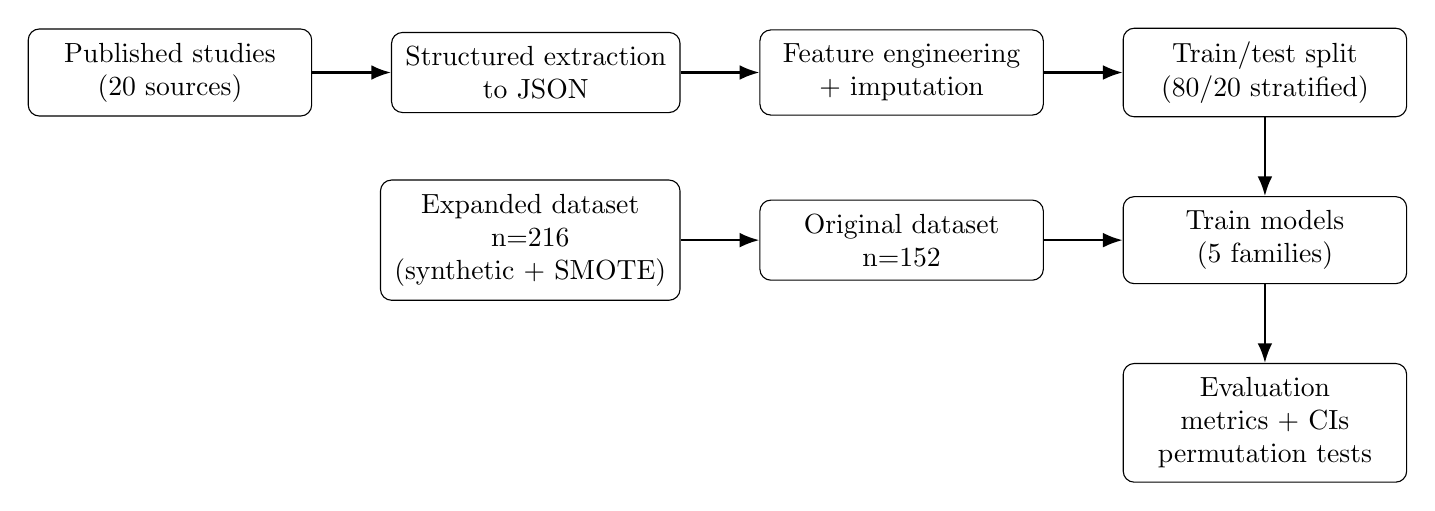
\begin{tikzpicture}[
  node distance=10mm,
  box/.style={draw, rounded corners, align=center, inner sep=5pt, minimum width=36mm},
  arrow/.style={-{Latex[length=2.5mm]}, thick}
]
\node[box] (lit) {Published studies\\(20 sources)};
\node[box, right=of lit] (json) {Structured extraction\\to JSON};
\node[box, right=of json] (feat) {Feature engineering\\+ imputation};
\node[box, right=of feat] (split) {Train/test split\\(80/20 stratified)};
\node[box, below=of split] (train) {Train models\\(5 families)};
\node[box, left=of train] (orig) {Original dataset\\n=152};
\node[box, left=of orig] (exp) {Expanded dataset\\n=216\\(synthetic + SMOTE)};
\node[box, below=of train] (eval) {Evaluation\\metrics + CIs\\permutation tests};

\draw[arrow] (lit) -- (json);
\draw[arrow] (json) -- (feat);
\draw[arrow] (feat) -- (split);
\draw[arrow] (split) -- (train);
\draw[arrow] (orig) -- (train);
\draw[arrow] (exp) -- (orig);
\draw[arrow] (train) -- (eval);
\end{tikzpicture}
\caption{MEN2 Predictor workflow from cohort assembly to benchmarking across original and expanded datasets, with automatic confidence interval calculation for all models.}
\end{figure}

\begin{figure}[ht]
\centering
\includegraphics[width=\linewidth]{../charts/variant_distribution.png}
\caption{Distribution of RET variants in the paper-only cohort (n = 152).}
\end{figure}

\begin{figure}[ht]
\centering
\includegraphics[width=\linewidth]{../charts/age_histograms.png}
\caption{Age distribution of RET carriers in the paper-only cohort.}
\end{figure}

\begin{figure}[ht]
\centering
\includegraphics[width=\linewidth]{../charts/calcitonin_cea_relationship.png}
\caption{Observed calcitonin--CEA relationship across cohorts with paired measurements (n = 34).}
\end{figure}

\begin{figure}[ht]
\centering
\begin{subfigure}{0.49\linewidth}
\centering
\includegraphics[width=\linewidth]{../charts/roc_curves/logistic_regression_original.png}
\caption{Logistic Regression (Original)}
\end{subfigure}
\begin{subfigure}{0.49\linewidth}
\centering
\includegraphics[width=\linewidth]{../charts/roc_curves/lightgbm_expanded.png}
\caption{LightGBM (Expanded)}
\end{subfigure}
\caption{Representative ROC curves for the zero-miss baseline (original logistic regression) and the highest-accuracy expanded model (LightGBM).}
\end{figure}

\begin{figure}[ht]
\centering
\begin{subfigure}{\linewidth}
\centering
\includegraphics[width=\linewidth]{../charts/confusion_matrices/logistic_regression_original.png}
\caption{Logistic Regression (Original)}
\end{subfigure}

\vspace{0.75\baselineskip}

\begin{subfigure}{\linewidth}
\centering
\includegraphics[width=\linewidth]{../charts/confusion_matrices/lightgbm_expanded.png}
\caption{LightGBM (Expanded)}
\end{subfigure}
\caption{Confusion matrices for representative models (raw and normalized panels are embedded in each figure).}
\end{figure}

\begin{figure}[ht]
\centering
\includegraphics[width=\linewidth]{../charts/shap/lightgbm/expanded_bar.png}
\caption{SHAP global feature importance (mean absolute SHAP) for LightGBM on the expanded dataset.}
\end{figure}

\begin{figure}[ht]
\centering
\includegraphics[width=\linewidth]{../charts/lime/lightgbm/lime_global_importance.png}
\caption{LIME global feature importance (mean absolute LIME weight) computed over representative explained cases for LightGBM.}
\end{figure}

\FloatBarrier

\section{Conclusion}
MEN2 Predictor presents a reproducible machine learning workflow for rare-disease risk stratification by aggregating published MEN2/RET-carrier evidence into a structured dataset and standardized evaluation pipeline. On the literature-derived cohort of 152 confirmed RET carriers spanning 24 variants (ATA risk levels 1--3), the original paper-only logistic regression baseline achieved 100\% recall with 70.97\% accuracy, supporting its use as a conservative ``zero-miss'' screening-oriented model where sensitivity is prioritized over overall accuracy.

In a case-control setting (n = 1{,}069 total records) using variant-matched synthetic controls and SMOTE applied to training folds, LightGBM achieved the highest accuracy (97.20\%) with 96.08\% recall. These results suggest that augmentation can improve discrimination for triage-style use, but recall volatility remains a critical risk in safety-sensitive workflows where missed cancers are unacceptable.

Key limitations include the cohort size, heterogeneity across published sources, and biomarker missingness requiring imputation. Prospective external validation is required before clinical deployment. Overall, MEN2 Predictor is best positioned as a screening and prioritization aid that complements, rather than replaces, genetic testing and guideline-based care.

\textbf{Clinical disclaimer:} This work and the accompanying software are provided for research and educational purposes only. They are not medical advice and must not be used as a diagnostic tool or as a substitute for clinician judgment, guideline-based evaluation, and confirmatory genetic testing.

\FloatBarrier

\section*{Acknowledgements}
We thank the authors of the contributing studies for publishing detailed clinical reports that enable secondary analyses in rare-disease research.


We also thank Ms Unnati Saxena for mentoring support and for coordinating and facilitating the project work.

We acknowledge the open-source community and software ecosystem that supported this work, including scikit-learn, numpy, and visualization libraries used to support reproducible analysis.

\clearpage
\FloatBarrier
\section*{References}
\printbibliography[heading=none]

\clearpage
\appendix
\renewcommand{\thefigure}{S\arabic{figure}}
\renewcommand{\thetable}{S\arabic{table}}
\setcounter{figure}{0}
\setcounter{table}{0}

\section{Supplementary Materials}
\subsection{Study Composition}
% Auto-generated from data/raw/literature_data.json
\begin{longtable}{@{}p{0.78\linewidth}p{0.18\linewidth}@{}}
\caption{RET-carrier counts by source study label used in the aggregated cohort (total n=152).} \\
\toprule
Study label & Patients (n) \\
\midrule
\endfirsthead
\toprule
Study label & Patients (n) \\
\midrule
\endhead
European Journal of Endocrinology (2006) & 46 \\
Thyroid Journal (2016) & 24 \\
JCEM (2022) ctDNA Cohort & 21 \\
Oncotarget (2015) RET S891A FMTC & 15 \\
Indian Journal of Cancer (2021) RET S891A Family & 7 \\
Clinics and Practice (2024) RET C634G Kindred & 6 \\
JCEM (2018) Homozygous RET K666N & 6 \\
Endocrinol. Diabetes Metab. Case Reports (2024) RET K666N & 4 \\
JCEM Case Reports (2025) & 4 \\
Laryngoscope (2021) MEN2A Penetrance & 4 \\
World Journal of Clinical Cases (2024) RET C634Y Family & 3 \\
Annals of Medicine \& Surgery (2025) RET C634R Case & 2 \\
Genes (2022) RET c.1901G>A Family & 2 \\
Surgery Today (2014) RET S891A Pheo & 2 \\
AJCR (2022) Calcitonin-Negative MTC & 1 \\
Annales d'Endocrinologie (2015) RET Y791F & 1 \\
BMC Pediatrics (2020) MEN2B Case & 1 \\
Case Reports in Endocrinology (2020) RET Exon 11 delins & 1 \\
Case Reports in Medicine (2012) MEN2B & 1 \\
JCEM (2016) RET Exon 7 Deletion & 1 \\
\bottomrule
\end{longtable}


Supplementary figures are available in the project GitHub repository at \url{https://github.com/arjuncodess/men2-predictor} under \texttt{charts/}.

An interactive demonstration (Gradio web app) and a programmatic API are also available via the Hugging Face Space at \url{https://huggingface.co/spaces/arjuncodess/men2-predictor}. The hosted Space is provided as-is for demonstration only and must not be used for clinical decision-making.

\end{document}
